\chapter{title}
\newpage
\begin{abox}
	Practise Set-1
\end{abox}
\begin{enumerate}[label=\color{ocre}\textbf{\arabic*.}]
	\item An unbiased dice is thrown three times successively. The probability that the numbers of dots on the uppermost surface add up to 16 is
{\exyear{NET/JRF(DEC-2011)}}
\begin{tasks}(4)
	\task[\textbf{A.}] $\frac{1}{16}$
	\task[\textbf{B.}] $\frac{1}{36}$
	\task[\textbf{C.}] $\frac{1}{108}$
	\task[\textbf{D.}] $\frac{1}{216}$
\end{tasks}
\item A ball is picked at random from one of two boxes that contain 2 black and 3 white and 3 black and 4 white balls respectively. What is the probability that it is white?
{\exyear{NET/JRF(JUNE-2012)}}
\begin{tasks}(4)
	\task[\textbf{A.}] $34 / 70$
	\task[\textbf{B.}] $41 / 70$
	\task[\textbf{C.}] $36 / 70$
	\task[\textbf{D.}] $29 / 70$
\end{tasks}
\item  A bag contains many balls, each with a number painted on it. There are exactly $n$ balls which have the number $n$ (namely one ball with 1 , two balls with 2, and so on until $N$ on them). An experiment consists of choosing a ball at random, noting the number on it and returning it to the bag. If the experiment is repeated a large number of times, the average value the number will tend to
{\exyear{NET/JRF(JUNE-2012)}}
\begin{tasks}(4)
	\task[\textbf{A.}] $\frac{2 N+1}{3}$
	\task[\textbf{B.}] $\frac{N}{2}$
	\task[\textbf{C.}] $\frac{N+1}{2}$
	\task[\textbf{D.}] $\frac{N(N+1)}{2}$
\end{tasks}
\item  In a series of five Cricket matches, one of the captains calls "Heads" every time when the toss is taken. The probability that he will win 3 times and lose 2 times is
{\exyear{NET/JRF(DEC-2012)}}
\begin{tasks}(4)
	\task[\textbf{A.}] $1 / 8$
	\task[\textbf{B.}]  $5 / 8$
	\task[\textbf{C.}] $3 / 16$
	\task[\textbf{D.}] $5 / 16$
\end{tasks}
\item  Two independent random variables $m$ and $n$, which can take the integer values $0,1,2, \ldots, \infty$, follow the Poisson distribution, with distinct mean values $\mu$ and $v$ respectively. Then
{\exyear{NET/JRF(DEC-2014)}}
\begin{tasks}(1)
	\task[\textbf{A.}]  The probability distribution of the random variable $l=m+n$ is a binomial distribution.
	\task[\textbf{B.}] The probability distribution of the random variable $r=m-n$ is also a Poisson distribution.
	\task[\textbf{C.}] The variance of the random variable $l=m+n$ is equal to $\mu+v$
	\task[\textbf{D.}] The mean value of the random variable $r=m-n$ is equal to 0 
\end{tasks}
\item  Consider a random walker on a square lattice. At each step the walker moves to a nearest neighbour site with equal probability for each of the four sites. The walker starts at the origin and takes 3 steps. The probability that during this walk no site is visited more than one is
{\exyear{NET/JRF(DEC-2015)}}
\begin{tasks}(4)
	\task[\textbf{A.}] $12 / 27$
	\task[\textbf{B.}] $27 / 64$
	\task[\textbf{C.}] $3 / 8$
	\task[\textbf{D.}] $9 / 16$
\end{tasks}
\item  Let $X$ and $Y$ be two independent random variables, each of which follow a normal distribution with the same standard deviation $\sigma$, but with means $+\mu$ and $-\mu$, respectively. Then the sum $X+Y$ follows a
{\exyear{NET/JRF(JUNE-2016)}}
\begin{tasks}(1)
	\task[\textbf{A.}] Distribution with two peaks at $\pm \mu$ and mean 0 and standard deviation $\sigma \sqrt{2}$
	\task[\textbf{B.}]  Normal distribution with mean 0 and standard deviation $2 \sigma$
	\task[\textbf{C.}] Distribution with two peaks at $\pm \mu$ and mean 0 and standard deviation $2 \sigma$
	\task[\textbf{D.}] Normal distribution with mean 0 and standard deviation $\sigma \sqrt{2}$
\end{tasks}
\item  A random variable $n$ obeys Poisson statistics. The probability of finding $n=0$ is $10^{-6}$. The expectation value of $n$ is nearest to
{\exyear{NET/JRF(JUNE-2017)}}
\begin{tasks}(4)
	\task[\textbf{A.}] 14
	\task[\textbf{B.}] $10^{6}$
	\task[\textbf{C.}] $e$
	\task[\textbf{D.}] $10^{2}$
\end{tasks}
\item At each time step, a random walker in one dimension either remains at the same point with probability $\frac{1}{4}$, or moves by a distance $\Delta$ to the right or left with probabilities $\frac{3}{8}$ each. After $N$ time steps, its root mean squared displacement is
{\exyear{NET/JRF(JUNE-2019)}}
\begin{tasks}(4)
	\task[\textbf{A.}] $\Delta \sqrt{N}$
	\task[\textbf{B.}] $\Delta \sqrt{\frac{9 N}{16}}$
	\task[\textbf{C.}] $\Delta \sqrt{\frac{3 N}{4}}$
	\task[\textbf{D.}] $\Delta \sqrt{\frac{3 N}{8}}$
\end{tasks}
\item A box contains 5 white and 4 black balls. Two balls are picked together at random from the box. What is the probability that these two balls are of different colours?
{\exyear{NET/JRF(DEC-2019)}}
\begin{tasks}(4)
	\task[\textbf{A.}] $\frac{1}{2}$ 
	\task[\textbf{B.}] $\frac{5}{18}$
	\task[\textbf{C.}] $\frac{1}{3}$
	\task[\textbf{D.}] $\frac{5}{9}$
\end{tasks}
\item  A particle hops randomly from a site to its nearest neighbour in each step on a square lattice of unit lattice constant. The probability of hopping to the positive $x$-direction is $0.3$, to the negative $x$-direction is $0.2$, to the positive $y$-direction is $0.2$ and to the negative $y$-direction is $0.3 .$ If a particle starts from the origin, its mean position after $N$ steps is
{\exyear{NET/JRF(DEC-2019)}}
\begin{tasks}(4)
	\task[\textbf{A.}] $\frac{1}{10} N(-\hat{i}+\hat{j})$
	\task[\textbf{B.}] $\frac{1}{10} N(\hat{i}-\hat{j})$
	\task[\textbf{C.}] $N(0.3 \hat{i}-0.2 \hat{j})$
	\task[\textbf{D.}] $N(0.2 \hat{i}-0.3 \hat{j})$
\end{tasks}
\item A basket consists of an infinite number of red and black balls in the proportion $p:(1-p)$. Three balls are drawn at random without replacement. The probability of their being two red and one black is a maximum for
{\exyear{NET/JRF(JUNE-2020)}}
\begin{tasks}(4)
	\task[\textbf{A.}]  $p=\frac{3}{4}$
	\task[\textbf{B.}] $p=\frac{3}{5}$
	\task[\textbf{C.}] $p=\frac{1}{2}$
	\task[\textbf{D.}] $p=\frac{2}{3}$
\end{tasks}
\end{enumerate}
 \colorlet{ocre1}{ocre!70!}
\colorlet{ocrel}{ocre!30!}
\setlength\arrayrulewidth{1pt}
\begin{table}[H]
	\centering
	\arrayrulecolor{ocre}
	\begin{tabular}{|p{1.5cm}|p{1.5cm}||p{1.5cm}|p{1.5cm}|}
		\hline
		\multicolumn{4}{|c|}{\textbf{Answer key}}\\\hline\hline
		\rowcolor{ocrel}Q.No.&Answer&Q.No.&Answer\\\hline
		1&\textbf{B} &2&\textbf{B}\\\hline 
		3&\textbf{A} &4&\textbf{D} \\\hline
		5&\textbf{C} &6&\textbf{D} \\\hline
		7&\textbf{D}&8&\textbf{A}\\\hline
		9&\textbf{C}&10&\textbf{D}\\\hline
		11&\textbf{B} &12&\textbf{D}\\\hline
		
	\end{tabular}
\end{table}

\newpage
\begin{abox}
	Practise Set-2
\end{abox}
\begin{enumerate}[label=\color{ocre}\textbf{\arabic*.}]
		\item An unbiased die is cast twice. The probability that the positive difference (bigger smaller) between the two numbers is 2 is
	{\exyear{ JEST 2012}}
	\begin{tasks}(2)
		\task[\textbf{a.}]$\frac{1}{9}$
		\task[\textbf{b.}]$\frac{2}{9}$
		\task[\textbf{c.}] $\frac{1}{6}$
		\task[\textbf{d.}] $\frac{1}{3}$
	\end{tasks}
	\item A box contains 100 coins out of which 99 are fair coins and 1 is a double-headed coin. Suppose you choose a coin at random and toss it 3 times. It turns out that the results of all 3 tosses are heads. What is the probability that the coin you have drawn is the doubleheaded one?
	{\exyear{ JEST 2013}}
	\begin{tasks}(2)
		\task[\textbf{a.}] $0.99$
		\task[\textbf{b.}]$0.925$
		\task[\textbf{c.}] $0.75$
		\task[\textbf{d.}] $0.01$
	\end{tasks}
	\item There are on average 20 buses per hour at a point, but at random times. The probability that there are no buses in five minutes is closest to
	{\exyear{ JEST 2013}}
	\begin{tasks}(2)
		\task[\textbf{a.}]$0.07$
		\task[\textbf{b.}] $0.60$
		\task[\textbf{c.}]$0.36$
		\task[\textbf{d.}] $0.19$
	\end{tasks}
	\item Two drunks start out together at the origin, each having equal probability of making a step simultaneously to the left or right along the $x$ axis. The probability that they meet after $n$ steps is
	{\exyear{ JEST 2013}}
	\begin{tasks}(2)
		\task[\textbf{a.}]$\frac{1}{4^{n}} \frac{2 n !}{n !^{2}}$
		\task[\textbf{b.}] $\frac{1}{2^{n}} \frac{2 n !}{n !^{2}}$
		\task[\textbf{c.}] $\frac{1}{2^{n}} 2 n !$
		\task[\textbf{d.}]  $\frac{1}{4^{n}} n !$
	\end{tasks}
	\item If two ideal dice are rolled once, what is the probability of getting atleast one '6'?
	{\exyear{ JEST 2015}}
	\begin{tasks}(2)
		\task[\textbf{a.}]$\frac{11}{36}$
		\task[\textbf{b.}]$\frac{1}{36}$
		\task[\textbf{c.}]$\frac{10}{36}$
		\task[\textbf{d.}]  $\frac{5}{36}$
	\end{tasks}
	\item The mean value of random variable $x$ with probability density $p(x)=\frac{1}{\sigma \sqrt{2 \pi}} . \exp \left[-\frac{\left(x^{2}+\mu x\right)}{\left(2 \sigma^{2}\right)}\right]$ is:
	{\exyear{ JEST 2016}}
	\begin{tasks}(2)
		\task[\textbf{a.}]0
		\task[\textbf{b.}]$\frac{\mu}{2}$
		\task[\textbf{c.}] $\frac{-\mu}{2}$
		\task[\textbf{d.}]  $\sigma$
	\end{tasks}
	\item Suppose that we toss two fair coins hundred times each. The probability that the same number of heads occur for both coins at the end of the experiment is
	{\exyear{ JEST 2017}}
	\begin{tasks}(2)
		\task[\textbf{a.}]$\left(\frac{1}{4}\right)^{100} \sum_{n=0}^{100}\left(\begin{array}{c}100 \\ n\end{array}\right)$
		\task[\textbf{b.}] $2\left(\frac{1}{4}\right)^{100} \sum_{n=0}^{100}\left(\begin{array}{c}100 \\ n\end{array}\right)^{2}$
		\task[\textbf{c.}]$\frac{1}{2}\left(\frac{1}{4}\right)^{100} \sum_{n=0}^{100}\left(\begin{array}{c}100 \\ n\end{array}\right)^{2}$
		\task[\textbf{d.}] $\left(\frac{1}{4}\right)^{100} \sum_{n=0}^{100}\left(\begin{array}{c}100 \\ n\end{array}\right)^{2}$
	\end{tasks}
	\item An electronic circuit with 10000 components performs its intended function success fully with a probability $0.99$ if there are no faulty components in the circuit. The probability that there are faulty components is $0.05$. if there are faulty components, the circuit perform successfully with a probability $0.3$. The probability that the circuit performs successfully is $\frac{x}{10000}$. What is $x$ ?
	{\exyear{ JEST 2018}}
	\item A person plans to go from town $A$ to town $B$ by taking either the route $(R 1+R 2)$ with probability $\frac{1}{2}$ or the route $(R 1+R 3)$ with probability $\frac{1}{2}$ (see figure). Further, there is a probability $\frac{1}{3}$ that $R 1$ is blocked, a probability $\frac{1}{3}$ that $R 2$ is blocked, and a probability $\frac{1}{3}$ that $R 3$ is blocked. What is the probability that he/she would reach town $B$ ?
	{\exyear{ JEST 2019}}
	\begin{figure}[H]
		\centering
		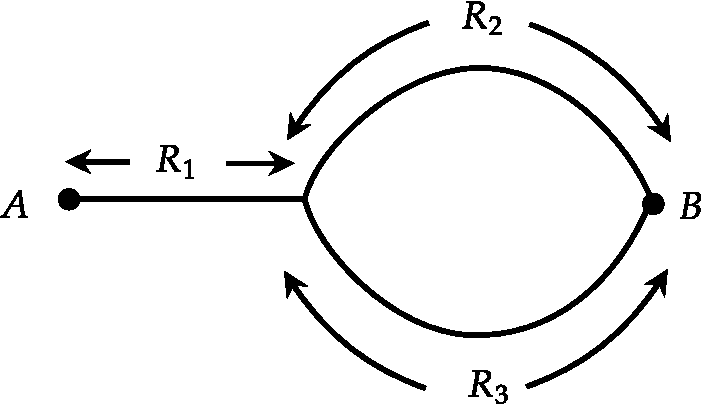
\includegraphics[height=3cm,width=5.5cm]{JEST-58-2019}
	\end{figure}
	\begin{tasks}(2)
		\task[\textbf{a.}]$\frac{8}{9}$
		\task[\textbf{b.}]$\frac{1}{3}$
		\task[\textbf{c.}]$\frac{4}{9}$
		\task[\textbf{d.}]$\frac{2}{3}$
	\end{tasks}
\end{enumerate}
 \colorlet{ocre1}{ocre!70!}
\colorlet{ocrel}{ocre!30!}
\setlength\arrayrulewidth{1pt}
\begin{table}[H]
	\centering
	\arrayrulecolor{ocre}
	\begin{tabular}{|p{1.5cm}|p{1.5cm}||p{1.5cm}|p{1.5cm}|}
		\hline
		\multicolumn{4}{|c|}{\textbf{Answer key}}\\\hline\hline
		\rowcolor{ocrel}Q.No.&Answer&Q.No.&Answer\\\hline
		1&\textbf{B} &2&\textbf{C}\\\hline 
		3&\textbf{D} &4&\textbf{A} \\\hline
		5&\textbf{A} &6&\textbf{A} \\\hline
		7&\textbf{D}&8&\textbf{9555(NAT)}\\\hline
		9&\textbf{C}&&\textbf{}\\\hline
		
	\end{tabular}
\end{table}
